\newpage
\section{Rectas paralelas y perpendiculares}

El análisis de líneas rectas puede visto desde varias ramas de la matemática, 
en este caso lo veremos desde el lado de la geometría euclídeana. Sin embargo,
es necesario destacar que se puede analizar también desde la geometría 
analítica, por lo tanto es posible tener varias definiciones de un concepto, 
sin que estas sen contrapongan.

%TODO:- Introducir el concepto de semi recta

\subsection{Paralelismo}

\marginnote{Cuando dos o más figuras geométricas se cortan (es decir, tienen 
puntos en común) se dice que se \textbf{intersecan}}

\begin{definition}
  Los rectas son \textbf{paraleas} en un plano si nunca se \textbf{intersectan} 
  y siempre guardan la misma distancia una de otra.
  \begin{center}
    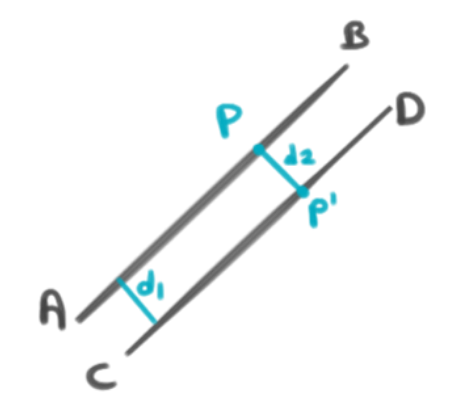
\includegraphics[width=4cm]{paralelas}
  \end{center}
  En la imagen podemos observar que $d_1 = d_ 2$, por lo tanto $\overline{AB}$ y 
  $\overline{CD}$ son paralelas.\\

  La condición de paralelismo se simboliza de matemática como:
  \[\overline{AB} \parallel \overline{CD}\]
  donde 
  \begin{itemize}
    \item [$\overline{AB}$] es el segmento AB
    \item [$\overline{CD}$] es el segmento CD
    \item [$\parallel$] es el simbolo de paralelismo
  \end{itemize}
\end{definition}

\subsubsection{El quinto postulado de Euclides}

El \textbf{quinto postulado de Euclides} estable que \textit{Data  
\textcolor{blue}{una recta} cualquiera, y \textcolor{orange}{un punto} 
fuera de ella, existe una y solo una recta paralela a la inicial, que pase 
por dicho punto}.

\subsection{Perpendicularidad}

\marginnote{El cuadrado en AOC indica un ángulo de $90^\circ$}

\begin{definition}
  Las rectas \textbf{perpendiculares} son aquellas que al intersectarse forman 
  un ángulo de $90^\circ$.
  \begin{center}
    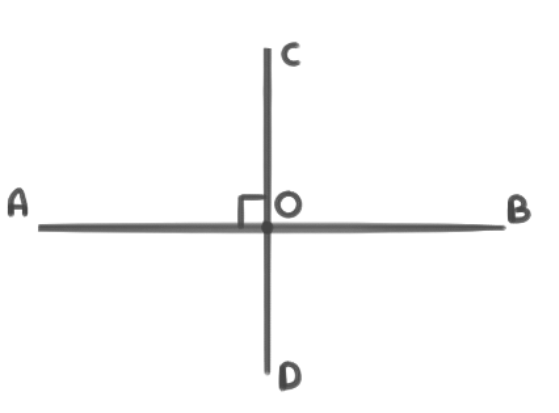
\includegraphics[width=4cm]{perpendicularidad}
  \end{center}
  La condición de perpendicularidad se simboliza de matemática como:
  \[\overline{AB} \perp \overline{CD}\]
  donde 
  \begin{itemize}
    \item [$\overline{AB}$] es el segmento AB
    \item [$\overline{CD}$] es el segmento CD
    \item [$\perp$] es el simbolo de perpendicularidad
  \end{itemize}

  En realidad, se forman 4 ángulos rectos ($90^\circ$), sin embargo, con que se 
  verifique la existencia de un ángulo recto basta.

\end{definition}

\subsubsection{Rectas oblicuas}

Por otra parte, si las rectas se intersecan en un ángulo \textbf{diferente} a 
$90^\circ$ se les conoce como \textbf{\textcolor{blue}{oblicuas}}

\subsection{Ángulos opuestos por el vértice}

Los ángulos opuestos por el vértice se forman con un par de rectas 
\sidenote{Algunos autores remarcan el hecho de que las rectas deber ser 
\textit{no paralelas}, sin embargo esto se puede obviar puesto que las rectas
deben tener un vértice en común.} tienen un vértice en común.

\begin{figure}[ht!]
	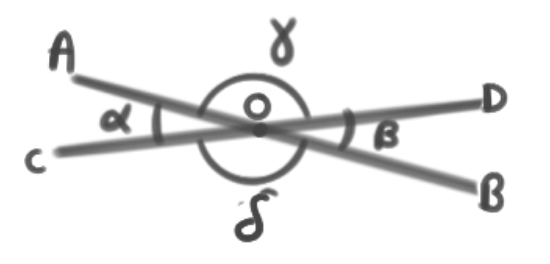
\includegraphics[width=7cm]{opporvertice}
	\caption[AngOpVertice]{Ángulos opuestos por el vértice.}
	\labfig{opporvertice}
\end{figure}

De la figura \reffig{opporvertice} se desprenden lo siguiente:
\begin{equation*}
\boxed{
\begin{array}{rcl}	
		\alpha &=& \beta \\
		\gamma &=& \delta 
	\end{array}
}
\end{equation*}

Las cuales se cumplen siempre para cualesquiera rectas con un vértice en común.

\textbf{¿Qué podrían preguntarnos en un examen? Veamos} \\

\textbf{NOTA:} Se recomienda tener nociones de aritmética y álgebra para revisar
los ejercicios propuestos.

\marginnote{\textbf{Recordatorio} \\ 
\begin{tabular}{c c}
  $\alpha + \beta = 90^\circ$ & 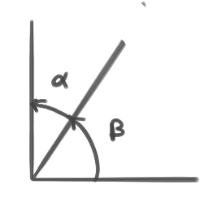
\includegraphics[width=1.5cm]{complementario} \\
	$\alpha + \beta = 180^\circ$ & 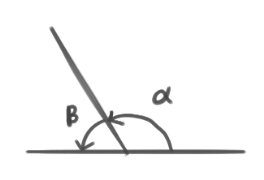
\includegraphics[width=2cm]{suplementario} \\ 
	$\alpha + \beta = 360^\circ$ & 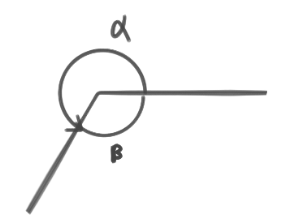
\includegraphics[width=2cm]{conjugado} 
\end{tabular}
}

\begin{example}
  Halla el valor de $x$ de la figura mostrada a continuación
  \begin{center}
    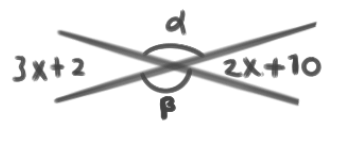
\includegraphics[width=5cm]{opvertEj01}
  \end{center}
  \textbf{Solución}. Por propiedades de ángulos opuesto por el vértice:
  \begin{equation*}
    \begin{array}{rcl}	
        3x + 2 & = & 2x + 10
    \end{array}
  \end{equation*}
  Y lo que resta es simplemente despejar $x$ por medio del álgebra
  \begin{align*}
      3x + 2 - 2x & = 10 \\
      3x - 2x & = 10 - 2 \\
      \Aboxed{x & = 8}
  \end{align*} 
  Eso quiere decir que el ángulo que mide $3x +2$ es igual a 
  \[3(8) + 2 = 26^\circ\]
\end{example}

\subsection{Ángulos adyacentes}

Se considera que dos ángulos son adyacentes si estos son contiguos 
(esta uno al lado del otro) y además, la suma de estos es igual a $180^\circ$.

\begin{figure}[ht!]
	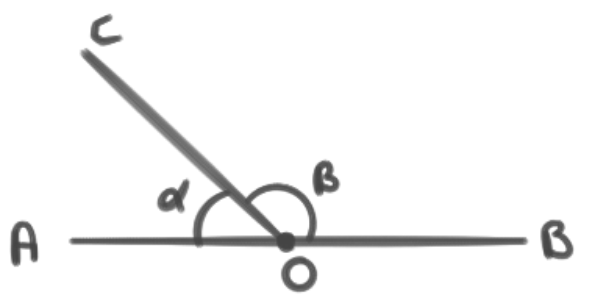
\includegraphics[width=6cm]{adyacente}
	\caption[AngAdyacentes]{Ángulos adyacentes.}
	\labfig{adyacente}
\end{figure}

De la figura \reffig{adyacente} se observa que 
\[\boxed{\alpha + \beta = 180^\circ}\]

\begin{example}
  Del ejemplo anterior, cuya figura se vuelve a mostar
  \begin{center}
    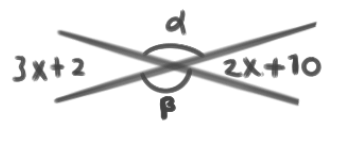
\includegraphics[width=5cm]{opvertEj01}
  \end{center}
  Hallar el valor de $\alpha$ y de $\beta$\\
  \textbf{Solución} 
  \[(3x +2) + \alpha = 180^\circ\]
  
  Ya conocemos el valor de $(3x +2)$ es igual a $26^\circ$ 
  \[\therefore (3x +2) + \alpha = 
    \textcolor{blue}{26^\circ} + \alpha = 180^\circ\]

  Despejando en valor de $\alpha$, se obtiene
  \begin{align*}
    \alpha & = 180^\circ - 26^\circ \\
    \therefore\; \Aboxed{\alpha & = 154^\circ } \\
  \end{align*}

\end{example}

\subsection{Rectas paralelas cortadas por una secante}

Los conceptos que veremos a continuación (ángulos interntos, externo y alternos)
nacen a partir del  análisis de \underline{dos rectas paralelas y otra oblicua},
que las corta y se conoce cómo \textit{secante}.

\begin{figure}[ht!]
	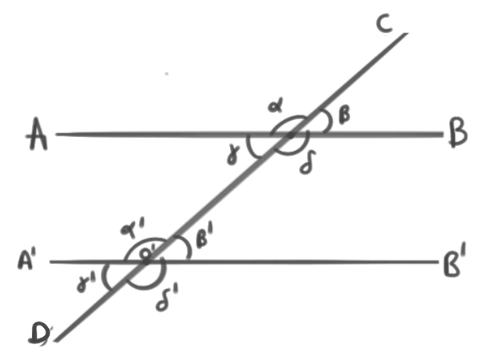
\includegraphics[width=9cm]{rectparalysec}
	\caption[RectasParalelas]{Rectas paralelas cortadas por una secante.
    \begin{itemize}
      \item $\overline{AB} \parallel \overline{A'B'}$
      \item $\overline{CD}$ es la recta \textit{secante}
    \end{itemize}
  }
	\labfig{rectparalysec}
\end{figure}

Como se observa en la figura \reffig{rectparalysec}, se producen \textit{dos} 
puntos de intersección, llamados $O$ y $O'$, producto de la recta secante con 
las paralelas.
\begin{itemize}
  \item Se generan \textit{4 ángulos} por cada intersección.
  \item Es decir, en total tenemos \textit{8 ángulos}.
\end{itemize}

Para identificar cada ángulo los nombraremos con base en lo siguiente:\\

\textbf{De acuerdo a su posición}

\begin{itemize}
  \item \textbf{Internos.} Son ángulos que están entre (o dentro) de las dos
    rectas paralelas.\\
    En la figura son: $\pmb{\gamma}$, $\pmb{\delta}$, 
    $\pmb{\alpha}'$, $\pmb{\beta}'$
  \item \textbf{Externos.} Son aquellos que están fuera de entre las dos rectas,
    es decir, están en la parte del plano que no esta comprendida entre las 
    rectas.\\
    En la figura son: $\pmb{\alpha}$, $\pmb{\beta}$, $\pmb{\gamma'}$, 
    $\pmb{\delta'}$
\end{itemize}

\textbf{De acuerdo a su referencia: con respecto a otro ángulo 
  y a la recta secante
}

Los ángulos que se mencionan a continuación se dan en pares y los varios son 
siempre los mismos. Por ejemplo en el caso de los anternos 
$\pmb{\alpha}$ = $\pmb{\delta'}$

\begin{itemize}
  \item \textbf{Alternos.} Dos ángulos son alternos si están en 
    \textit{lados opuestos} de la recta secante. Además ambos son 
    \textit{externos} o \textit{internos}.\\
    % y no comparten niguno de su lados. \\
    En la figura son:
    \begin{itemize}
      \item $\pmb{\alpha}$ y $\pmb{\delta'}$
      \item $\pmb{\beta}$ y $\pmb{\gamma'}$
      \item $\pmb{\gamma}$ y $\pmb{\beta'}$
      \item $\pmb{\delta}$ y $\pmb{\alpha'}$
    \end{itemize}
  \item \textbf{Conjugados.} Dos ángulos son correspondientes si están en el 
    \textit{mismo lado} de la recta secante y ambos son \textit{externos} o
    \textit{internos}.\\
    En la figura son:
    \begin{itemize}
      \item Para el lado izquierdo:
      \begin{itemize}
        \item $\pmb{\alpha}$ y $\pmb{\gamma}$
        \item $\pmb{\alpha'}$ y $\pmb{\gamma'}$
      \end{itemize}
      \item Para el lado derecho:
      \begin{itemize}
        \item $\pmb{\beta}$ y $\pmb{\delta}$
        \item $\pmb{\beta'}$ y $\pmb{\delta'}$
      \end{itemize}
    \end{itemize}
  \item \textbf{Correpondientes.} Dos ángulos son correspondientes si están del
    \textit{mismo lado} de la secante, uno es \textit{externo} y otro 
    \textit{interno}.\\
    % y no comparten ninguno de sus lados.\\
    En la figura son: 
    \begin{itemize}
      \item $\pmb{\alpha}$ y $\pmb{\alpha'}$
      \item $\pmb{\beta}$ y $\pmb{\beta'}$
      \item $\pmb{\gamma}$ y $\pmb{\gamma'}$
      \item $\pmb{\delta}$ y $\pmb{\delta'}$
    \end{itemize}
\end{itemize}

\textbf{De acuerdo a su posición y a su referencia}

\begin{marginfigure}[-6cm]
	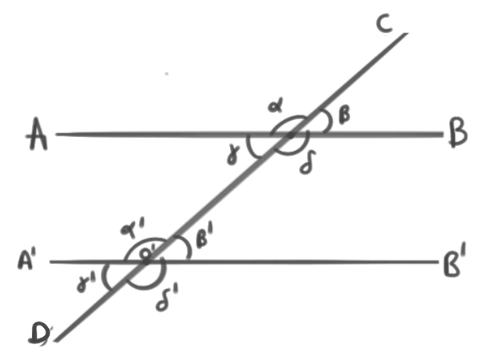
\includegraphics{rectparalysec}
	\caption[rectparalysec]{Rectas paralelas cortadas por una secante. En resumen
	  \begin{itemize}
      \item Ángulos alternos internos:
      \begin{itemize}
        \item $\pmb{\gamma} = \pmb{\beta'}$
        \item $\pmb{\delta} = \pmb{\alpha'}$
      \end{itemize}
      \item Ángulos alternos externos:
      \begin{itemize}
        \item $\pmb{\alpha} = \pmb{\delta'}$
        \item $\pmb{\beta} = \pmb{\gamma'}$
      \end{itemize}
      \item Ángulos correspondientes:
      \begin{itemize}
        \item $\pmb{\alpha} = \pmb{\alpha'}$
        \item $\pmb{\beta} = \pmb{\beta'}$
        \item $\pmb{\gamma} = \pmb{\gamma'}$
        \item $\pmb{\delta} = \pmb{\delta'}$
      \end{itemize}
    \end{itemize}
  }
	\labfig{pythagoras}
\end{marginfigure}

A la hora de habla de rectas cortadas por una secante \textit{lo más común} es 
referirse a los ángulos por su posición y su referencia.
Los siguiente ángulos se nombrar con base en us posición y referencia, como en 
el caso anterior, vienen el pares y su valor es el mismo:

\begin{itemize}
  \item \textbf{Ángulos alternos internos}. Son aquellos ángulos internos y que 
    a la vez son alternos.\\
    En la figura son: 
    \begin{itemize}
      \item $\pmb{\gamma}$ y $\pmb{\beta'}$
      \item $\pmb{\delta}$ y $\pmb{\alpha'}$
    \end{itemize}
    
  \item \textbf{Ángulos alternos externos}. Son ángulos que son externos y a la 
  vez alternos.\\
  En la figura son:
  \begin{itemize}
    \item $\pmb{\alpha}$ y $\pmb{\delta'}$
    \item $\pmb{\beta}$ y $\pmb{\gamma'}$
  \end{itemize}

  \item \textbf{Ángulos colaterales internos}. La suma de dos ángulos internos 
    situados del mismo lado de la secante da $180^\circ$.\\
    En la figura: 
    \begin{itemize}
      \item $\pmb{\gamma} + \pmb{\alpha'} = 180^\circ$
      \item $\pmb{\delta} + \pmb{\beta'} = 180^\circ$
    \end{itemize}

  \item \textbf{Ángulos colaterales externos}. La suma de dos ángulos externos 
    situados del mismo lado de la secante da $180^\circ$.\\  
    En la figura: 
    \begin{itemize}
      \item $\pmb{\alpha} + \pmb{\gamma'} = 180^\circ$
      \item $\pmb{\beta} + \pmb{\delta'} = 180^\circ$
    \end{itemize}
\end{itemize}

\begin{example}
  Hallar el valor de $x$ y de los 8 ángulos de la figura 
  \begin{center}
    \begin{tikzpicture}[scale=0.6]
      \node (cp) at (60:1) {};
      \node (cp2) at (-1,0) {};
      \draw (-3,0) coordinate (a) node[left] {$A$} -- 
      (0,0) coordinate (o) -- 
      (3,0) coordinate (b) node[right] {$B$};
      \draw (60:2) coordinate (d) node[right]{$D$} -- 
        (60:-5) coordinate (c) node[right,below] {$C$};
      \pic["$\alpha$",draw=orange,->,angle eccentricity=1.5,angle radius=5mm] 
        {angle=b--o--cp};
      \pic["$2x-20^\circ$",draw=blue,->,angle eccentricity=1.5,angle radius=5mm] 
        {angle=cp--o--a};   
      \pic["$\gamma$",draw=orange,->,angle eccentricity=1.5,angle radius=5mm] 
        {angle=a--o--c};   
      \pic["$\delta$",draw=blue,->,angle eccentricity=1.5,angle radius=5mm] 
        {angle=c--o--b};        
      % Parte de abajo    
      \draw (-4,-3) coordinate (a2) node[left] {$A'$} -- 
      (-1.7,-3) coordinate (o2) -- 
      (2,-3) coordinate (b2) node[right] {$B'$};  
      \pic["$\alpha$'",draw=orange,->,angle eccentricity=1.6,angle radius=5mm] 
        {angle=b2--o2--d}; 
      \pic["$\beta$'",draw=blue,->,angle eccentricity=1.2,angle radius=5mm] 
        {angle=d--o2--a2};   
      \pic["$2x$",draw=orange,->,angle eccentricity=1.6,angle radius=5mm] 
        {angle=a2--o2--c};  
      \pic["$\delta$'",draw=blue,->,angle eccentricity=1.5,angle radius=5mm] 
        {angle=c--o2--b2};            
    \end{tikzpicture}
  \end{center}
\end{example}

\newpage % This is not right

\begin{figure*}[ht!]
  \begin{kaoexercises}
    Encontrar \textit{todos} los ángulos faltantes
    \begin{multicols*}{2}
      \begin{enumerate}
        % 1
        \item \textbf{}\\
        \begin{tikzpicture}[scale=0.7]
  \coordinate (o) at (0,0);
  \draw (o) -- (20:3) coordinate (a) node[right,above] {$A$};
  \draw (o) -- (160:3) coordinate (b) node[left,above] {$B$};
  \draw (o) -- (160:-3) coordinate (c) node[right,below] {$C$};
  \draw (o) -- (20:-3) coordinate (d) node[left,below] {$D$};
  \pic["$4x+34^\circ$'",draw=blue,->,angle eccentricity=1.5,angle radius=5mm] 
  {angle=a--o--b};    
  \pic["$\beta$",draw=orange,->,angle eccentricity=1.6,angle radius=5mm] 
  {angle=b--o--d};  
  \pic["$6x +12^\circ$'",draw=blue,->,angle eccentricity=1.5,angle radius=5mm] 
  {angle=d--o--c};  
  \pic["$\delta$",draw=orange,->,angle eccentricity=1.6,angle radius=5mm] 
  {angle=c--o--a};        
\end{tikzpicture}

        % 2
        \item \textbf{}\\
        \begin{tikzpicture}[scale=0.7]
  \coordinate (o) at (0,0);
  \draw (o) -- (20:3) coordinate (a) node[right,above] {$A$};
  \draw (o) -- (160:3) coordinate (b) node[left,above] {$B$};
  \draw (o) -- (160:-3) coordinate (c) node[right,below] {$C$};
  \draw (o) -- (20:-3) coordinate (d) node[left,below] {$D$};
  \pic["$x+12^\circ$",draw=blue,->,angle eccentricity=1.5,angle radius=5mm] 
  {angle=a--o--b};    
  \pic["$x-4^\circ$",draw=orange,->,angle eccentricity=2.3,angle radius=5mm] 
  {angle=b--o--d};  
  \pic["$\gamma$",draw=blue,->,angle eccentricity=1.5,angle radius=5mm] 
  {angle=d--o--c};  
  \pic["$\delta$'",draw=orange,->,angle eccentricity=1.5,angle radius=5mm] 
  {angle=c--o--a};        
\end{tikzpicture} 

        % 3
        \item \textbf{}\\
        \begin{tikzpicture}[scale=0.5]
  \node (cp) at (60:1) {};
  \node (cp2) at (-1,0) {};
  \draw (-3,0) coordinate (a) node[left] {$A$} -- 
  (0,0) coordinate (o) -- 
  (3,0) coordinate (b) node[right] {$B$};
  \draw (60:2) coordinate (d) node[right]{$D$} -- 
    (60:-5) coordinate (c) node[right,below] {$C$};
  \pic["$\alpha$",draw=orange,->,angle eccentricity=1.5,angle radius=5mm] 
    {angle=b--o--cp};
  \pic["$3x-6^\circ$",draw=blue,->,angle eccentricity=1.6,angle radius=5mm] 
    {angle=cp--o--a};   
  \pic["$\gamma$",draw=orange,->,angle eccentricity=1.5,angle radius=5mm] 
    {angle=a--o--c};   
  \pic["$\delta$",draw=blue,->,angle eccentricity=1.5,angle radius=5mm] 
    {angle=c--o--b};        
  % Parte de abajo    
  \draw (-4,-3) coordinate (a2) node[left] {$A'$} -- 
  (-1.7,-3) coordinate (o2) -- 
  (2,-3) coordinate (b2) node[right] {$B'$};  
  \pic["$\alpha$'",draw=orange,->,angle eccentricity=1.6,angle radius=5mm] 
    {angle=b2--o2--d}; 
  \pic["$\beta$'",draw=blue,->,angle eccentricity=1.2,angle radius=5mm] 
    {angle=d--o2--a2};   
  \pic["$x$",draw=orange,->,angle eccentricity=1.6,angle radius=5mm] 
    {angle=a2--o2--c};  
  \pic["$\delta$'",draw=blue,->,angle eccentricity=1.5,angle radius=5mm] 
    {angle=c--o2--b2};            
\end{tikzpicture}  

        % 4
        \item \textbf{}\\
        \begin{tikzpicture}[scale=0.5]
  \draw (-3,0) coordinate (a) node[left] {$A$} -- 
  (0,0) coordinate (o) -- 
  (3,0) coordinate (b) node[right] {$B$};
  \draw (120:2) coordinate (d) node[right]{$D$} -- 
    (120:-5) coordinate (c) node[right,below] {$C$};
  \pic["$\alpha$",draw=orange,->,angle eccentricity=1.5,angle radius=5mm] 
    {angle=b--o--d};
  \pic["$\beta$",draw=blue,->,angle eccentricity=2,angle radius=5mm] 
    {angle=d--o--a};   
  \pic["$2x+20^\circ$",draw=orange,->,angle eccentricity=1.6,angle radius=5mm] 
    {angle=a--o--c};   
  \pic["$\delta$",draw=blue,->,angle eccentricity=1.5,angle radius=5mm] 
    {angle=c--o--b};        
  % Parte de abajo    
  \draw (-2,-3) coordinate (a2) node[left] {$A'$} -- 
  (2,-3) coordinate (o2) -- 
  (4,-3) coordinate (b2) node[right] {$B'$};  
  \pic["$2x-5^\circ$'",draw=orange,->,angle eccentricity=1.6,angle radius=5mm] 
    {angle=b2--o2--d}; 
  \pic["$\beta$'",draw=blue,->,angle eccentricity=1.3,angle radius=5mm] 
    {angle=d--o2--a2};   
  \pic["$\gamma'$",draw=orange,->,angle eccentricity=1.6,angle radius=5mm] 
    {angle=a2--o2--c};  
  \pic["$\delta$'",draw=blue,->,angle eccentricity=1.5,angle radius=5mm] 
    {angle=c--o2--b2};            
\end{tikzpicture}            

        % 5
        \item \textbf{}\\
        \begin{tikzpicture}[scale=0.5]
  \draw (-3,0) coordinate (a) node[left] {$A$} -- 
  (0,0) coordinate (o) -- 
  (3,0) coordinate (b) node[right] {$B$};
  \draw (40:2) coordinate (d) node[right]{$D$} -- 
    (40:-6) coordinate (c) node[right,below] {$C$};
  \pic["$\alpha$",draw=orange,->,angle eccentricity=1.5,angle radius=5mm] 
    {angle=b--o--d};
  \pic["$\beta$",draw=blue,->,angle eccentricity=1.5,angle radius=5mm] 
    {angle=d--o--a};   
  \pic["$2x$",draw=orange,->,angle eccentricity=1.5,angle radius=5mm] 
    {angle=a--o--c};   
  \pic["$\delta$",draw=blue,->,angle eccentricity=1.5,angle radius=5mm] 
    {angle=c--o--b};        
  % Parte de abajo    
  \draw (-6,-3) coordinate (a2) node[left] {$A'$} -- 
  (-3.3,-3) coordinate (o2) -- 
  (1,-3) coordinate (b2) node[right] {$B'$};  
  \pic["$\alpha'$",draw=orange,->,angle eccentricity=1.6,angle radius=5mm] 
    {angle=b2--o2--d}; 
  \pic["$4x+24^\circ$",draw=blue,->,angle eccentricity=1.4,angle radius=5mm] 
    {angle=d--o2--a2};   
  \pic["$\gamma'$",draw=orange,->,angle eccentricity=1.6,angle radius=5mm] 
    {angle=a2--o2--c};  
  \pic["$\delta'$",draw=blue,->,angle eccentricity=1.5,angle radius=5mm] 
    {angle=c--o2--b2};            
\end{tikzpicture}             
        \columnbreak%
        % 6
        \item \textbf{}\\
        \begin{tikzpicture}[scale=0.5]
  \draw (-3,0) coordinate (a) node[left] {$A$} -- 
  (0,0) coordinate (o) -- 
  (3,0) coordinate (b) node[right] {$B$};
  \draw (140:2) coordinate (d) node[right]{$D$} -- 
    (140:-6.5) coordinate (c) node[right,below] {$C$};
  \pic["$\alpha$",draw=orange,->,angle eccentricity=1.5,angle radius=5mm] 
    {angle=b--o--d};
  \pic["$\beta$",draw=blue,->,angle eccentricity=2,angle radius=5mm] 
    {angle=d--o--a};   
  \pic["$\gamma$",draw=orange,->,angle eccentricity=1.5,angle radius=5mm] 
    {angle=a--o--c};   
  \pic["$2x$",draw=blue,->,angle eccentricity=1.5,angle radius=5mm] 
    {angle=c--o--b};        
  % Parte de abajo    
  \draw (0,-3) coordinate (a2) node[left] {$A'$} -- 
  (3.5,-3) coordinate (o2) -- 
  (5.5,-3) coordinate (b2) node[right] {$B'$};  
  \pic["$x+60^\circ$'",draw=orange,->,angle eccentricity=1.6,angle radius=5mm] 
    {angle=b2--o2--d}; 
  \pic["$\beta$'",draw=blue,->,angle eccentricity=1.4,angle radius=5mm] 
    {angle=d--o2--a2};   
  \pic["$y-10^\circ$",draw=orange,->,angle eccentricity=1.6,angle radius=5mm] 
    {angle=a2--o2--c};  
  \pic["$\delta$'",draw=blue,->,angle eccentricity=1.5,angle radius=5mm] 
    {angle=c--o2--b2};            
\end{tikzpicture}             

        % 7
        \item \textbf{}\\
        \begin{tikzpicture}[scale=0.5]
  \coordinate (a) at (0,0) node {$A$};
  \coordinate (o1) at (4,0);
  \coordinate (o2) at (8,0);
  \coordinate (b) at (12,0);
  \draw (a) -- (o1) -- (o2) -- (b) node {$B$};
  \draw (o1) -- +(60:3) coordinate (c) node[above] {$L1$};
  \draw (o1) -- +(60:-3) coordinate (d);
  \draw (o2) -- +(60:3) coordinate (e) node[above] {$L2$};
  \draw (o2) -- +(60:-3) coordinate (f);
  \pic["$\alpha$",draw=blue,->,angle eccentricity=1.5,angle radius=5mm] 
    {angle=c--o1--a}; 
  \pic["$2x-12^\circ$",draw=orange,->,angle eccentricity=2.1,angle radius=6mm] 
    {angle=a--o1--d};   
  \pic["$\gamma$",draw=blue,->,angle eccentricity=1.5,angle radius=5mm] 
    {angle=d--o1--b}; 
  \pic["$\delta$",draw=orange,->,angle eccentricity=1.5,angle radius=5mm] 
    {angle=b--o1--c};  
  \pic["$\alpha'$",draw=blue,->,angle eccentricity=1.5,angle radius=5mm] 
    {angle=e--o2--a}; 
  \pic["$\beta'$",draw=orange,->,angle eccentricity=1.5,angle radius=5mm] 
    {angle=a--o2--f};   
  \pic["$\gamma'$",draw=blue,->,angle eccentricity=1.5,angle radius=5mm] 
    {angle=f--o2--b}; 
  \pic["$2x+10^\circ$",draw=orange,->,angle eccentricity=2.4,angle radius=6mm] 
    {angle=b--o2--e};                          
\end{tikzpicture}           
      
        % 8
        \item \textbf{}\\
        \begin{tikzpicture}[scale=0.5]
  \coordinate (a) at (0,0) node[left] {$A$};
  \coordinate (o1) at (4,0);
  \coordinate (o2) at (8,0);
  \coordinate (b) at (12,0);
  \draw (a) -- (o1) -- (o2) -- (b) node[right] {$B$};
  \draw (o1) -- +(120:3) coordinate (c) node[above] {$L1$};
  \draw (o1) -- +(120:-3) coordinate (d);
  \draw (o2) -- +(120:3) coordinate (e) node[above] {$L2$};
  \draw (o2) -- +(120:-3) coordinate (f);
  \pic["$x$",draw=blue,->,angle eccentricity=1.5,angle radius=5mm] 
    {angle=c--o1--a}; 
  \pic["$\beta$",draw=orange,->,angle eccentricity=1.6,angle radius=5mm] 
    {angle=a--o1--d};   
  \pic["$\gamma$",draw=blue,->,angle eccentricity=1.5,angle radius=5mm] 
    {angle=d--o1--b}; 
  \pic["$\delta$",draw=orange,->,angle eccentricity=1.5,angle radius=5mm] 
    {angle=b--o1--c};  
  \pic["$\alpha'$",draw=blue,->,angle eccentricity=1.5,angle radius=5mm] 
    {angle=e--o2--a}; 
  \pic["$\beta'$",draw=orange,->,angle eccentricity=1.6,angle radius=5mm] 
    {angle=a--o2--f};   
  \pic["$\gamma'$",draw=blue,->,angle eccentricity=1.5,angle radius=5mm] 
    {angle=f--o2--b}; 
  \pic["$4x-30^\circ$",draw=orange,->,angle eccentricity=1.7,angle radius=5mm] 
    {angle=b--o2--e};                          
\end{tikzpicture}           

        % 9
        \item \textbf{}\\
        \begin{tikzpicture}[scale=0.5]
  \coordinate (a) at (0,0) node[left] {$A$};
  \coordinate (o1) at (4,1);
  \coordinate (o2) at (8,2);
  \coordinate (b) at (12,3);
  \draw (a) -- (o1) -- (o2) -- (b) node[right] {$B$};
  \draw (o1) -- +(120:3) coordinate (c) node[above] {$L1$};
  \draw (o1) -- +(120:-3) coordinate (d);
  \draw (o2) -- +(120:3) coordinate (e) node[above] {$L2$};
  \draw (o2) -- +(120:-3) coordinate (f);
  \pic["$3x+15^\circ$",draw=blue,->,angle eccentricity=2.5,angle radius=5mm] 
    {angle=c--o1--a}; 
  \pic["$\beta$",draw=orange,->,angle eccentricity=1.5,angle radius=5mm] 
    {angle=a--o1--d};   
  \pic["$\gamma$",draw=blue,->,angle eccentricity=1.5,angle radius=5mm] 
    {angle=d--o1--b}; 
  \pic["$\delta$",draw=orange,->,angle eccentricity=1.5,angle radius=5mm] 
    {angle=b--o1--c};  
  \pic["$\alpha'$",draw=blue,->,angle eccentricity=1.5,angle radius=5mm] 
    {angle=e--o2--a}; 
  \pic["$\beta'$",draw=orange,->,angle eccentricity=1.5,angle radius=5mm] 
    {angle=a--o2--f};   
  \pic["$2x+20^\circ$",draw=blue,->,angle eccentricity=2.8,angle radius=5mm] 
    {angle=f--o2--b}; 
  \pic["$\delta'$",draw=orange,->,angle eccentricity=1.5,angle radius=5mm] 
    {angle=b--o2--e};                          
\end{tikzpicture}                
        % 10
        \item \textbf{}\\
        \begin{tikzpicture}[scale=0.5]
  \coordinate (a) at (0,3);
  \coordinate (o1) at (4,2);
  \coordinate (o2) at (8,1);
  \coordinate (b) at (12,0);
  \draw (a) node[left] {$A$} -- (o1) -- (o2) -- (b) node[right] {$B$};
  \draw (o1) -- +(45:3) coordinate (c) node[above] {$L1$};
  \draw (o1) -- +(45:-3) coordinate (d);
  \draw (o2) -- +(45:3) coordinate (e) node[above] {$L2$};
  \draw (o2) -- +(45:-3) coordinate (f);
  \pic["$4x-24^\circ$",draw=blue,->,angle eccentricity=2,angle radius=5mm] 
    {angle=c--o1--a}; 
  \pic["$\beta$",draw=orange,->,angle eccentricity=1.5,angle radius=5mm] 
    {angle=a--o1--d};   
  \pic["$\gamma$",draw=blue,->,angle eccentricity=1.5,angle radius=5mm] 
    {angle=d--o1--b}; 
  \pic["$\delta$",draw=orange,->,angle eccentricity=1.5,angle radius=5mm] 
    {angle=b--o1--c};  
  \pic["$\alpha'$",draw=blue,->,angle eccentricity=1.5,angle radius=5mm] 
    {angle=e--o2--a}; 
  \pic["$\beta'$",draw=orange,->,angle eccentricity=1.5,angle radius=5mm] 
    {angle=a--o2--f};   
  \pic["$\gamma'$",draw=blue,->,angle eccentricity=1.5,angle radius=5mm] 
    {angle=f--o2--b}; 
  \pic["$2x-12^\circ$",draw=orange,->,angle eccentricity=2.6,angle radius=5mm] 
    {angle=b--o2--e};                          
\end{tikzpicture}                         
      \end{enumerate}
    \end{multicols*}
  \end{kaoexercises}
\end{figure*}

%TODO:- Historia de Eratóstenes

% PSEUDO BIBLIOGRAFIA
% https://edu.gcfglobal.org/es/geometria-basica/posicion-relativa-de-rectas/1/
% https://edu.gcfglobal.org/es/geometria-basica/
%   rectas-paralelas-cortadas-por-una-secante/1/